%\documentclass{aip-cp}
\documentclass[%
aip,
% jmp,
% bmf,
% sd,
% rsi,
cp,  % Conference Proceedings
amsmath,amssymb,%nobibnotes,
% preprint,%
reprint,%
%author-year,%
%author-numerical,%
]{revtex4-2}

\usepackage{graphicx}% Include figure files
\usepackage{dcolumn}% Align table columns on decimal point
\usepackage{bm}% bold math
%\usepackage[mathlines]{lineno}% Enable numbering of text and display math
%\linenumbers\relax % Commence numbering lines

\usepackage[utf8]{inputenc}
\usepackage[T1]{fontenc}
%% Loads a Times-like font. You can also load
%% {newtxtext,newtxtmath}, but not {times}, 
%% {txfonts} nor {mathtpm} as these packages
%% are obsolete and have been known to cause problems.
\usepackage{mathptmx} 

\usepackage{xcolor}

\usepackage{caption}
%\usepackage{hyperref}
%\hypersetup{colorlinks = true,
%            linkcolor = blue,
%            urlcolor  = blue,
%            citecolor = red,
%            anchorcolor = blue}

\usepackage{subcaption}

\usepackage{listings}

\definecolor{codegreen}{rgb}{0,0.6,0}
\definecolor{codegray}{rgb}{0.5,0.5,0.5}
\definecolor{codepurple}{rgb}{0.58,0,0.82}
\definecolor{backcolour}{rgb}{0.95,0.95,0.92}

\lstdefinestyle{mystyle}{
	backgroundcolor=\color{backcolour},  
	commentstyle=\color{codegreen},
	keywordstyle=\color{magenta},
	numberstyle=\tiny\color{codegray},
	stringstyle=\color{codepurple},
	basicstyle=\footnotesize,
	breakatwhitespace=false,        
	breaklines=true,                
	captionpos=b,                   
	keepspaces=true,                
	numbers=left,                   
	numbersep=5pt,                 
	showspaces=false,               
	showstringspaces=false,
	showtabs=false,                 
	tabsize=2
}

\lstset{style=mystyle}


%\usepackage[numbers]{natbib}
%%\usepackage[
%%backend=biber, 
%%style=authoryear,
%%url=false, 
%%doi=true
%%]{biblatex}
%%\addbibresource{RFPPC2019_Hillairet.bib}

\begin{document}
	
	\title{RF Network Analysis of the WEST ICRH Antenna with the Open-Source Python scikit-rf Package}
	
	\author{Julien Hillairet}
	\email[Corresponding author: ]{julien.hillairet@cea.fr}
	\affiliation{CEA, IRFM, F-13108 St-Paul-Lez-Durance, France}

	
	\begin{abstract}
		\texttt{Scikit-rf} is an open-source Python package developed for RF/Microwave engineering. The package provides a modern, object-oriented library for network analysis and calibration which is both flexible and scalable. Besides offering standard microwave network physics and operations, it is also capable of advanced operations such as interpolating between an individual set of networks or deriving network statistical properties. The package also allows direct plotting of rectangular plots, Smith Charts or automated uncertainty bounds. In this paper, the \texttt{scikit-rf} package is used to simulate the WEST ICRH antennas. The antenna is modelled by connecting the various elements that compose it, separately full-wave modelled. Tunable elements, such as the matching capacitors, can be either created from ideal lump components or from interpolating full-wave calculations performed at various capacitance configurations. Finally, a numerical antenna model of a WEST ICRH antenna can be used offline or online by using operating-system-level virtualization services.
	\end{abstract}
	
	\maketitle	
	
	\section{INTRODUCTION}
	Modern science is founded on hypothesis testing and statistical significances of its derived results. Reproducing experiments, experimental or numerical, is the reason why scientists can gain confidence in their conclusions. However, during the last decades, the number of codes and libraries developed at an individual or a laboratory scale only increased. When these tools are not open-sourced, it leads to an obvious reproducibility problem as one should only rely on authors claims. To conform to the necessity of reproducibility in science,  software sources used in physical and engineering researches should ideally be made open when possible \cite{Ince2012}. The case of RF network manipulation and analysis is no different.  
	
	\texttt{Scikit-rf}\footnote{www.scikit-rf.org} is a Python package produced for RF/Microwave engineering  \cite{Arsenovic2018}. The package is licensed under the Berkeley Software Distribution (BSD) licence and is actively developed by volunteers on GitHub. The package provides a modern, object-oriented library for RF network analysis and calibration. Besides offering standard microwave network operations, such as reading/writing Touchstone files (\texttt{.sNp}), connecting or de-embedding N-port networks, frequency/port slicing, concatenation or interpolations, it is also capable of advanced operations such as Vector Network Analyzer (VNA) calibrations, time-gating, interpolating between an individual set of networks, deriving network statistical properties and supports Virtual Instrument for direct communication to VNAs. The package also allows straightforward plotting of rectangular plots (dB, mag, phase, group delay, etc), Smith Charts or automated uncertainty bounds. As the package is developed in Python, it makes it naturally compatible with the rich and modern scientific Python libraries \cite{Millman2011}, for example  \texttt{scikit-learn} for machine learning tasks \cite{scikit-learn} or \texttt{PlasmaPy} \cite{PlasmaPyCommunity2018} for plasma physics. Using Jupyter notebooks documents\cite{Kluyver2016}, modelling approaches and results can be shared and even directly reproduced using tools such as Binder\footnote{https://mybinder.org/}\cite{project-jupyter-proc-scipy-2018} or Google Colab\footnote{https://colab.research.google.com/}, by other researchers (or future self) few months or years after work had been made.
	
	In this paper, some functionalities of the \texttt{scikit-rf} package are presented through the example of modelling the WEST (Tungsten-W Environment in Steady-state Tokamak) Ion Cyclotron Resonance Heating (ICRH) antenna. The antenna circuit is made by connecting the various elements that compose it, separately full-wave modelled or using equivalent lumped models, like done with proprietary codes (i.e. owned by the person or the firm who has developed it)  in \cite{Durodie2015, Helou2015SIDON} or with commercial software such as ANSYS Designer in \cite{Hillairet2015}. This paper is accompanied by Jupyter notebooks illustrating in more details the code leading to the results presented here\cite{Hillairet2019zenodo}.
	
	
	\section{WEST Antenna Matching Capacitors}
	The three WEST ICRH antennas are load tolerant resonant structures equipped with internal vacuum matching capacitors. These capacitors are tuned before the antenna operation or are real-time controlled to maintain low reflected power toward the RF sources \cite{Hillairet2015}. In order to forge a relevant numerical model of the antenna, it is thus needed to modify the capacitance of these matching capacitors. At least two approaches can be used: (i) using an equivalent lumped model of the capacitor or (ii) interpolating the capacitor s-parameters from full-wave simulations (if available). The challenge with the former is to use a relevant model to capture the RF behaviour of the capacitor in its operational environment, where parasitic capacitances/inductances may arise from surrounding elements and are mostly unknown. The main difficulty with the later is to design a full-wave parametrized model geometrically accurate, assuming dimensions and materials of the capacitor are known. Both approaches can be implemented with \texttt{scikit-rf} as the package is able to compute s-parameters of RF circuits made from ideal lumped elements (resistor/capacitor/inductor, in series/shunt configuration)  or to interpolate between N-port networks with same frequencies \footnote{Similar to the \texttt{NPort\_Multi} component in ANSYS Designer}. In the example below, both approaches are mixed: the capacitor (from COMET), which has been previously simulated with ANSYS HFSS for few different capacitance configurations in \cite{Helou2018PhD}, is used to extract the lumped element parameters. Once fitted to an equivalent model, the capacitor networks can be driven as a function of their capacitances, while s-parameter interpolation only depend on of geometrical parameter (like the distance between capacitor electrodes).
	
	A N-port electrical network is described in \texttt{scikit-rf} with the \texttt{Network} object, defined from its network parameters (s, z, y-parameters),
	port characteristic impedances and frequency information. It can be created from a file or directly from data. Importing all the touchstone files located in directory into a collection of \texttt{Network} in a \texttt{NetworkSet} object and plotting the real part of the $S_{21}$ parameter for each network for a subset of the frequency range is straightforward\footnote{Due to space constraints, the code snippets are complete minimal example but does not necessary reproduce all figure details such as line styles, markers or labels. Readers should refer to associated notebooks for the full code listing.}:
	
	\begin{lstlisting}[language=Python]
	import skrf as rf
	capas_set = rf.NetworkSet.from_dir('S_Matrices/Antenna/Capacitor')
	capas_set['20-80 MHz'].plot_s_re(m=1, n=0)  # Indexing starts at 0 in Python	\end{lstlisting}
	
	Assuming the \texttt{NetworkSet} contains $M$ networks coming from a parameter sweep of $M$ values described in a \texttt{param\_values} array, creating an interpolated network for a new value is achieved with:
	
	\begin{lstlisting}[language=Python]
	ntw = capas_set.interpolate_from_network(param_values, new_value)	\end{lstlisting}
	
	Figure~1(b) illustrates the interpolation of $S_{11}$ and $S_{21}$ at a given frequency for intermediate values of the swept parameter, here related to the distance between capacitor electrodes (noted $D_{cylinders}$). Obviously, the interpolation precision increases with the number of networks in the set.
	
	The equivalent lumped model proposed by the capacitor manufacturer (COMET) in the capacitor documentation consists in a RLC circuit (in parallel with a resistance $R_p$). 
	% with the capacitance $C$ tunable from 15 to 150 pF and the elements $L\leqslant 24$ nH and $R_p$ and $R_s$ in the order of 20 to 50 M$\Omega$ and 5-10 m$\Omega$ respectively.
	However, in the case of the WEST ICRH antenna, the capacitor is inserted inside the antenna and is surrounded by the outer conductor elements, creating additional stray capacitances and inductances. In this situation, its turns out that the equivalent capacitance of the setup is modified \cite{Helou2018PhD}. The RF capacitance can nevertheless be extracted from full-wave calculation using a refined equivalent lumped model with additional shunt capacitances and RL elements around the capacitor itself to model the proximity of the outer conductor housing and propagation effects\footnote{The parallel resistor $R_p$ can be neglected in the tens of MHz frequency range considered here.} (Figure \ref{fig:fig2}(a)). Such electrical network can be constructed with \texttt{scikit-rf} with the following function:
	
	\begin{lstlisting}[language=Python]
	def eq_capa(C, R, L, R1, C1, L1):  # here we neglect the parallel resistance R_p
		freq = rf.Frequency(start=5, stop=95, npoints=101, unit='MHz')
		line = rf.media.DefinedGammaZ0(frequency=freq, z0=50)  # ideal transmission line media
		pre  = line.resistor(R1) ** line.inductor(L1) ** line.shunt_capacitor(C1)
		post = line.shunt_capacitor(C1) ** line.resistor(R1) ** line.inductor(L1)
		capa = line.resistor(R) ** line.inductor(L) ** line.capacitor(C)
		return pre ** cap ** post  # ** is the scikit-rf network cascading operator	\end{lstlisting}
	
	Using the standard optimization toolbox shipped in the \texttt{scipy} package, the model parameters can be fitted for each full-wave network. Once done, full-wave references and lumped model can be compared. The Figure~\ref{fig:fig2}(b) shows the calculated $S_{21}$ parameter which fit nice with the reference full-wave values. For most capacitance configurations, the error is below -40~dB. Taking constant lumped parameters ($R_s, L_s, C_1=C_2, R_1=R_2, L_1=L_2$) but $C$, the still matches well the full-wave reference except for the lowest range of capacitance values, in a region where the relationship between the electrodes distance and the capacitance is no more linear. The model can thus be used to determine a realistic relationship between the RF capacitance and the capacitor configuration (driven by motors).
	
	\begin{figure*}
		\centering
		\begin{subfigure}[t]{0.49\textwidth}
			\centering
			
\includegraphics[width=.9\linewidth]{figures/capacitor_equivalent_circuit}
			\caption{equivalent lumped models of a WEST antenna matching capacitor, outside and inside the antenna.}
		\end{subfigure}%
		~
		\begin{subfigure}[t]{0.49\textwidth}
			\centering
			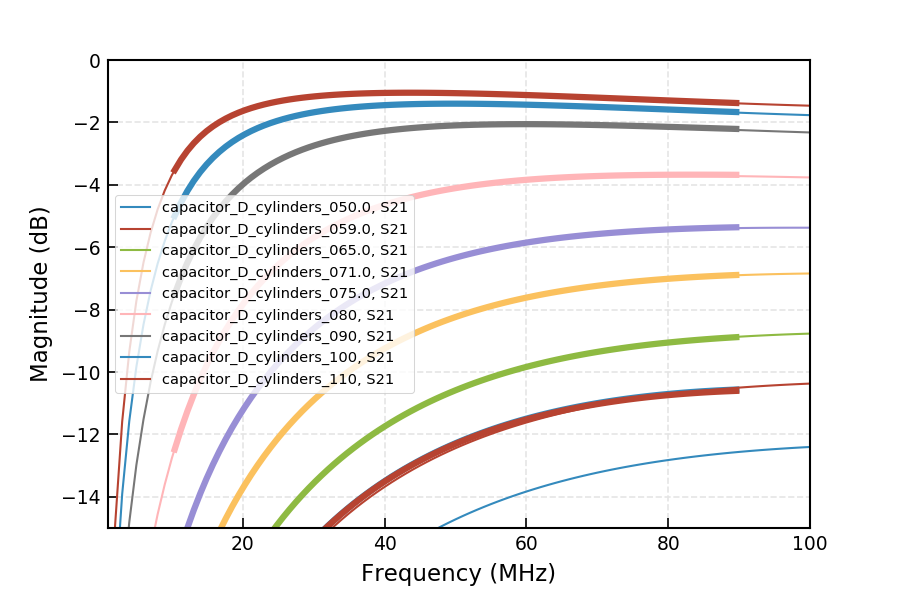
\includegraphics[width=.9\linewidth]{figures/comparison_fullwave_lumped_S21}
			\caption{Real part of $S_{21}$ between the reference from full-wave  calculations (thin lines) and the lumped model (thick lines).}
		\end{subfigure}
		\caption{Equivalent lumped model of the WEST ICRH antenna capacitor.}
		\label{fig:fig2}
	\end{figure*}
	
	\subsection{Antenna RF Circuit}
	In \texttt{scikit-rf}, there is at least two ways of building a RF circuit made of various networks, both illustrated in the accompanying notebooks. The first method consists in connecting networks one by one using \texttt{Network} methods. A second method consists in defining all the connections between networks and ports at once time, then use the \texttt{Circuit} object to build the resultant network. While the later method can be more verbose than the former, it has some advantages when the circuit has many connections. \texttt{Circuit} uses a systematic solving method giving both internal (for each circuit connections) and external (for ports) s-parameters for an arbitrary number of networks and interconnections and independently of the circuit excitation \cite{Hallbjorner2003}. By imposing excitations at ports, it allows obtaining voltages/currents inside the circuit.
	
	The Figure~\ref{fig:antenna_circuit} schematizes a half WEST ICRH antenna, where the impedances connected to the capacitors model the antenna loading. The associated \texttt{Circuit} is built from the code example given in Figure~\ref{fig:skrf_circuit_halfantenna}. In this example, each network has been previously imported or created. The Figure~\ref{fig:halfantennacurrentvoltage} illustrates the voltage and current at the capacitors, extracted from the circuit for a specified excitation. The full antenna, which consists in two adjacent similar circuits can be built similarly. \texttt{Circuit} allows visualizing the circuit graph using the \texttt{networkx} package \cite{Hagberg2008}, which is useful to check that the intended circuit is the one expected (such as connections, port numbers and characteristic impedances). The Figure~\ref{fig:antenna_graph} illustrates the full antenna setup loaded by a 4-port networks modelling the coupling of the antenna front-face to a plasma.
	
	\begin{minipage}{\textwidth}
		\begin{minipage}[b]{0.55\textwidth}
			\centering
			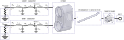
\includegraphics[width=.9\linewidth]{figures/antenna_circuit}
			
			\captionof{figure}{Half Antenna schematic.}
			\label{fig:antenna_circuit}
		\end{minipage}
		\hfill
		\begin{minipage}[b]{0.4\textwidth}
			\begin{lstlisting}[language=Python, basicstyle=\tiny]
connections = [
	[(port1, 0), (window, 0)],
	[(window, 1), (impedance_transformer, 0)],
	[(impedance_transformer, 1), (bridge, 0)],
	[(bridge, 1), (capa_upper, 0)],
	[(bridge, 2), (capa_lower, 0)],
	[(capa_upper, 1), (load_upper, 0)],
	[(capa_lower, 1), (load_lower, 0)],
	[(load_upper, 1), (ground_upper, 0)],
	[(load_lower, 1), (ground_lower, 0)]
]
# create the Circuit object and associated network
crt = rf.Circuit(connections) 
ntw = crt.network  # here a 1-port.			\end{lstlisting}
			\captionof{figure}{\texttt{scikit-rf Circuit} setup of an half-antenna.}
			\label{fig:skrf_circuit_halfantenna}
		\end{minipage}
	\end{minipage}
	
	\begin{minipage}{\textwidth}
		\begin{minipage}[b]{0.5\textwidth}
			\centering
			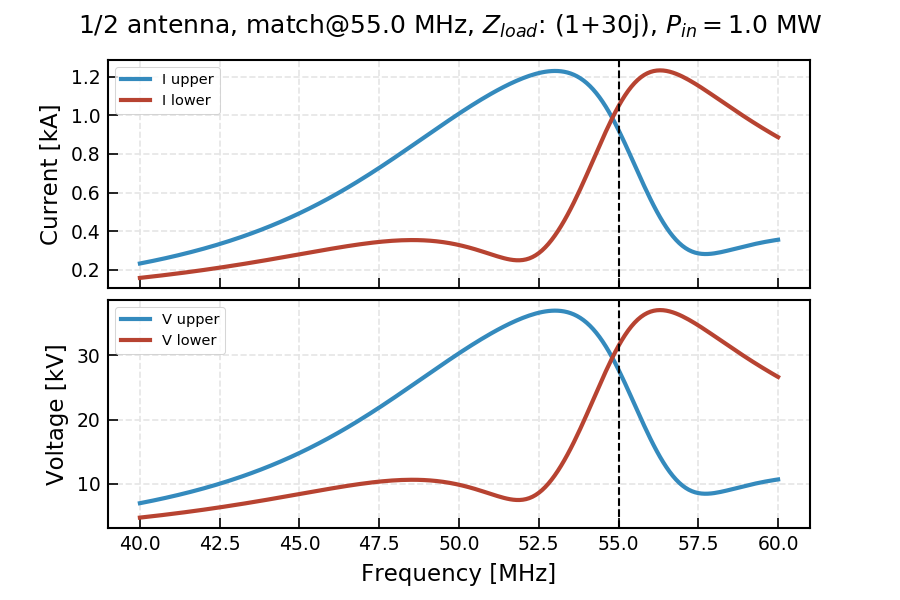
\includegraphics[width=.9\linewidth]{figures/half_antenna_current_voltage}
			\captionof{figure}{Voltages and currents at the matching capacitor for a defined power excitation, antenna loading and matching conditions.}
			\label{fig:halfantennacurrentvoltage}
		\end{minipage}
		\begin{minipage}[b]{0.5\textwidth}
			\centering
			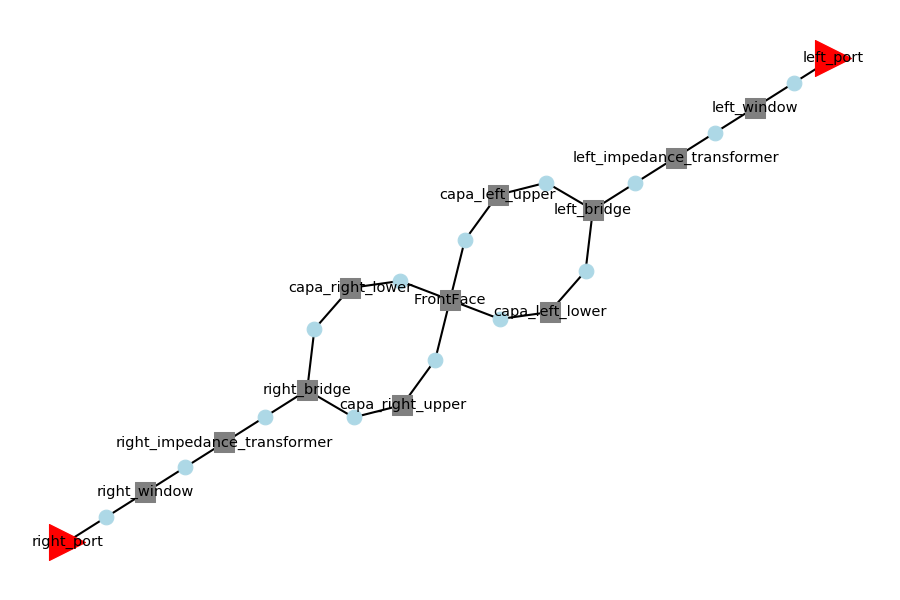
\includegraphics[width=.9\linewidth]{figures/antenna_graph}
			\captionof{figure}{Circuit graph of a complete antenna.}
			\label{fig:antenna_graph}
		\end{minipage}
	\end{minipage}
	
	
	\section{Conclusion}
	The RF circuit of the WEST ICRH antennas has been modelled using the open-source Python package \texttt{Scikit-rf}. The package provides a modern, object-oriented library for network analysis and calibration which is both flexible and scalable. As the package is developed in Python, it makes it naturally compatible with the rich and modern scientific Python libraries, testing and code coverage frameworks and reproducible modelling approaches using on-line virtualization services. The WEST ICRH antenna is modelled by connecting the various elements that compose it, separately full-wave modelled. Tunable elements, such as the matching capacitors, can be either created from ideal lump components or from interpolating full-wave calculations performed at various capacitance configurations. Being open-source, using \texttt{scikit-rf} to create the antenna numerical model with reproducible work-flow adds confidence in the fact that future users could use/maintain and extend it.
	
	
	\section{ACKNOWLEDGMENTS}
	The author would like to thank Alex Arsenovic and the  scikit-rf developers\footnote{https://github.com/scikit-rf/scikit-rf/graphs/contributors} for the scikit-rf package and their support. The capacitor full-wave model used to interpolate and extract lumped parameters had been made by W.Helou \cite{Helou2018PhD}.
	
	\bibliographystyle{aipnum-cp}%
	\bibliography{RFPPC2019_Hillairet}%
	
	
\end{document}